\scanpage{84}

fixant les arguments $t_j$ pour $j\ne i$, $L_k(t)=L_k(t_1,-t_n)$ \deleted{\unsure{devient|serait} \deleted{\illegible{1}} fonction linéaire strictement décroissante \deleted{\unsure{elle|$t_i$}} de $s=t_i$, majorée par la fonction continue croissante $\inserted{\varphi(\unsure{s|t})=}\varphi(t_1,-t_n)$, \deleted{\unsure{donc}} ce qui est manifestement impossible, \deleted{\unsure{puisque}}}\newline
\deleted{car $\unsure{\lambda_i|\lambda}$}\newline
\deleted{$\lambda(s)\to+\infty$ si $s\to-\infty$, et que $\varphi(s)$ reste borné pour $s\to-\infty$.}

on aurait $L(t)\to0$ si $t_i\to-\infty$, tandis que $\varphi(t)$ \deleted{\unsure{restant|resterait}}\inserted{resterait} borné pour $t_i\to-\infty$, ce \deleted{(\illegible{1} $\unsure{\varphi(t)}$} qui est incompatible avec $L(t)\leq\varphi(t)$ pour \deleted{tout} $t$. \deleted{\unsure{$f$}} Comme \deleted{\unsure{maintenant}}\inserted{enfin} $\varphi$ est aussi supposée symétrique, $L\deleted{\unsure{(t_1,-t_n)}}\leq\varphi\deleted{\unsure{(t_1,-t_n)}}$ \inserted{($L$ fonction sur $R^n$)} implique $\deleted{\unsure{L_k(t_{\sigma1},-t_{\sigma n})\leq\varphi(t_{\sigma1},\mathord{-}\,\mathord{-}t_{\sigma n})}}\inserted{\sigma L\leq\varphi}$ pour \deleted{tout} $\sigma\in\mathscr S_n$ (groupe des permutations des $n$ premiers entiers, i.e. \inserted{avec $\sigma L(t_1,-t_n)=L(t_{\sigma^{-1}1},\mathord{\cdot}\,\mathord{-}t_{\sigma^{-1}n})$}), donc on aura aussi

\[
\begin{array}{ll}
(7)&\displaystyle\deleted{\unsure{\varphi(t_1,-t_n)|\varphi(t)}}\varphi=\operatorname*{Sup}_k\operatorname*{Sup}_{\sigma\in\mathscr S_n}\sigma.L_k\deleted{\unsure{(t_1,-,t_n)}}
\end{array}
\]

Il s'ensuit que \deleted{\unsure{si}} pour prouver (1), il suffit de prouver que \inserted{pour $L\unsure{\in|=}L_k$, on a} \deleted{$\sigma L_k\deleted{\unsure{(\alpha_{\sigma1})}}\inserted{(\alpha_1,-\alpha_n)}\leq\varphi(\beta_1,-\beta_n)$ pour \deleted{tout} $k$, et tout $\sigma\in\mathscr S_n$. \unsure{Remplaçant|Remplaçons} \inserted{\deleted{\unsure{Désignant|Désignons}}} $L=$ $\sigma L_k$ par $L$, on est ramené à prouver}

\[
\begin{array}{ll}
(8)&\displaystyle\operatorname*{Sup}_{\sigma\in\mathscr S_n}(\sigma.L)(\alpha_1,\mathord{-}\,\mathord{\cdot}\alpha_n)\leq\operatorname*{Sup}_{\sigma\in\mathscr S_n}(\sigma L)(\beta_{\sigma1},\mathord{-}\,\mathord{-}\beta_{\unsure{\sigma n}})
\end{array}
\]

(car le deuxième mb en effet est $\leq\varphi(\beta_1,-\beta_n)$)\newline
\reversemarginpar\margin{\begin{tikzpicture}[x=1cm,y=1cm]\draw[red,line width=.4pt] (0,0)--(.02,.35);\end{tikzpicture}}\normalmarginpar
\begin{tikzpicture}[overlay,x=1cm,y=1cm]\draw[red,line width=.35pt] (0,-.22) .. controls (.45,-.38) and (.80,-.36) .. (1.25,-.28) .. controls (1.80,-.18) and (2.35,-.30) .. (2.90,-.29) .. controls (3.40,-.34) and (3.85,-.30) .. (4.20,-.24);\end{tikzpicture}
\deleted{\unsure{Pour le|Dans}}\inserted{Dans cette} inégalité, \deleted{\unsure{$L$ est une forme linéaire}} \inserted{$L(t_1,-t_n)=\sum_i^n a_it_i+b$}, \deleted{\unsure{affine et}} avec des \deleted{\unsure{$a_i$}} coefficients quelconques pour dans le cas b), et des $a_i>0$ pour tout $i$ dans le cas a) du lemme. \deleted{\inserted{\unsure{Désignons}} \unsure{Remarquons},} \inserted{On peut évidemment} \deleted{\unsure{résultat élémentaire} \unsure{bien} \illegible{1} \inserted{\unsure{Il suffit de démontrer que}}} supposer $b=0$.

\deleted{D'après un lemme connu, Il suffit \deleted{$\sum a_i\unsure{b_i}$} $L(\alpha_1,-,\alpha_n)\leq L(\quad$ \unsure{Notons que} $\sum a_i\alpha_i\leq\sum a_i\alpha_{\sigma i}$ quand $\sigma$ est une permutation telle que la suite des $a_{\sigma i}$ est \uline{décroissante}, ce qui}

D'après un lemme connu, \inserted{valable \unsure{donc puisque|du fait que} $\alpha_1\geq\alpha_2\geq-\geq\alpha_n$,} la somme $\sum a_{\sigma i}\alpha_i\inserted{=\sum a_i\alpha_{\sigma^{-1}i}}$ est maximum, pour $\sigma\in\mathscr S_n$ variable,

\reversemarginpar\margin{85}\normalmarginpar
